%%% LaTeX Template
%%% This template can be used for both articles and reports.
%%%
%%% Copyright: http://www.howtotex.com/
%%% Date: February 2011

%%% Preamble
\documentclass[paper=a4, fontsize=11pt]{scrartcl}	% Article class of KOMA-script with 11pt font and a4 format

\usepackage[margin=0.7in]{geometry}
\setcounter{secnumdepth}{4}

\usepackage[english]{babel}															% English language/hyphenation
\usepackage[protrusion=true,expansion=true]{microtype}				% Better typography
\usepackage{amsmath,amsfonts,amsthm}										% Math packages
\usepackage[pdftex]{graphicx}														% Enable pdflatex
\usepackage{seqsplit}
%\usepackage{color,transparent}													% If you use color and/or transparency
\usepackage[hang, small,labelfont=bf,up,textfont=it,up]{caption}	% Custom captions under/above floats
\usepackage{epstopdf}																	% Converts .eps to .pdf
\usepackage{subfig}																		% Subfigures
\usepackage{booktabs}																	% Nicer tables


%%% Advanced verbatim environment
\usepackage{verbatim}
\usepackage{fancyvrb}
\DefineShortVerb{\|}								% delimiter to display inline verbatim text


%%% Custom sectioning (sectsty package)
\usepackage{sectsty}								% Custom sectioning (see below)
\allsectionsfont{%									% Change font of al section commands
	\usefont{OT1}{bch}{b}{n}%					% bch-b-n: CharterBT-Bold font
%	\hspace{15pt}%									% Uncomment for indentation
	}

\sectionfont{%										% Change font of \section command
	\usefont{OT1}{bch}{b}{n}%					% bch-b-n: CharterBT-Bold font
	\sectionrule{0pt}{0pt}{-5pt}{0.8pt}%	% Horizontal rule below section
	}


%%% Custom headers/footers (fancyhdr package)
\usepackage{fancyhdr}
\pagestyle{fancyplain}
\fancyhead{}														% No page header
\fancyfoot[C]{\thepage}										% Pagenumbering at center of footer
\renewcommand{\headrulewidth}{0pt}				% Remove header underlines
\renewcommand{\footrulewidth}{0pt}				% Remove footer underlines
\setlength{\headheight}{13.6pt}

%%% Equation and float numbering
\numberwithin{equation}{section}															% Equationnumbering: section.eq#
\numberwithin{figure}{section}																% Figurenumbering: section.fig#
\numberwithin{table}{section}																% Tablenumbering: section.tab#
\usepackage[parfill]{parskip}
\usepackage{float}
\usepackage{graphicx}

%%% Title
\title{ \vspace{-1in} 	\usefont{OT1}{bch}{b}{n}
		\huge \strut An Overview of the Development of Indirect Inelastic Data Analysis in Mantid\strut \\
}
\author{ 									\usefont{OT1}{bch}{m}{n}
        Samuel Jackson\\		\usefont{OT1}{bch}{m}{n}
		ISIS Facility\\	\usefont{OT1}{bch}{m}{n}
        STFC Rutherford Appleton Laboratory\\
        \texttt{samuel.jackson@stfc.ac.uk}
}
\date{\today}

%%% Begin document
\begin{document}
\maketitle
\clearpage
\tableofcontents
\section{Introduction}
Mantid (http://www.mantidproject.org) is an open source, cross platform framework for the analysis of Neutron and Muon scattering data. The project is primarily written in C++ with a Python API. The project includes a GUI based off of the QtiPlot project and primarily written using the Qt library.

Mantid aims to provide a single platform for neutron and muon scattering data analysis to all facilities across the world. It is developed by two teams of developers, one based at the ISIS facility at Rutherford Appleton Laboratory UK, the other at the SNS facility at Oakridge USA. Recently additional partners from the ILL and PSI have also contributed.

The project is currently still under heavy development and provides regular incremental releases for evaluation and feedback from instrument scientists and users in general and is therefore constantly evolving with each release. Until recently, Mantid operated on a three month release cycle. This has now been changed to so that the project releases every four months, with a longer emphasis on the testing and integration phase of development.

Up until now the indirect inelastic section of Mantid has largely been based off of the the existing MODES application which in turn was based on OpenGenie\cite{wshowells2010}. The majority of the functionality has now been integrated into the Mantid framework in one form or another and we are now beginning to reach a point where we can expand the existing functionality further.

This document aims to give an overview of the current stage of development for the indirect inelastic section of the application as it currently exists in as much detail as possible to provide a historical snapshot of the progress so far. The remainder of the document then provides a weak outline of suggested directions for further development in the future.


\section{Indirect Geometry Instruments}

\section{Theory}
\mbox{ }\\
\begin{figure}[H]
\centering
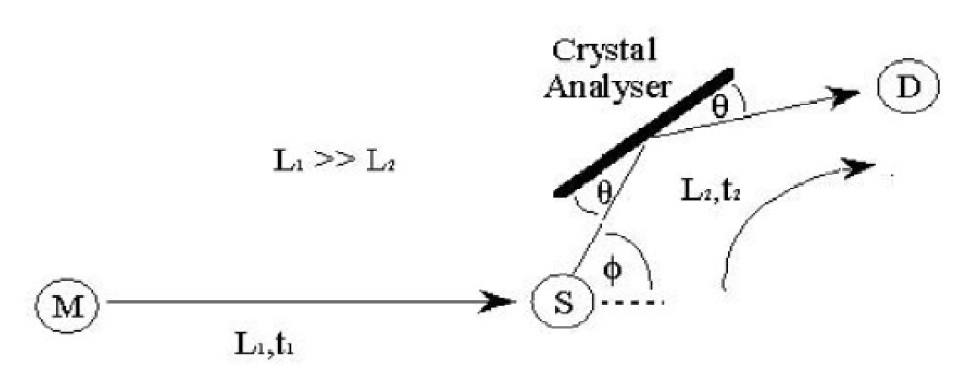
\includegraphics[width=0.7\textwidth]{img/instrument-diagram.png}
\caption{Diagram of the basic principle of an inelastic neutron scattering experiment. M is the moderator, S is the sample, and D is the detector \cite{smukhopadhyay2014}}
\label{fig:instrument-setup}
\end{figure}

In order to convert the raw data collected from the instrument from time of flight measurements to energy transfer the routine uses known parameters about the instrument as illustrated in figure \ref{fig:instrument-setup}. The final energy detected by a detector can be written in terms of a neutron's mass ($m_{n}$) and velocity ($v$) from the sample to the detector:

\begin{equation}
E_f = \frac{1}{2}m_{n}v^2 = \frac{1}{2}m_{n} ( L_2 / t_2 ) ^2
\end{equation}

Which can also be written in terms of the distance between sample and detector ($L_2$) and the time of flight $t_2$. To calculate the transfer of energy knowledge of the flight path between the moderator and sample ($L_1$) and the time of flight over this distance ($t_1$) can be used to calculate the incident energy using equation above. The transfer of energy is then simple the difference between incident and final energy:

\begin{equation}
\Delta E = E_i - E_f = \frac{1}{2}m_n[(L_1 / t_1-t_2)^2 - (L_1/t_2)^2]
\end{equation}

This is the fundamental principle behind the reduction routine described in the following section.
%\section{A Brief Introduction to Neutron Scattering}
%Neutron scattering experiments are used to probe the structure of materials at a fundamental level. The results of such experiments can be used to learn a great deal about the internal structure of a sample and how it can behave under different conditions. In a neutron scattering experiment, a beam of neutrons is produced at a source (such as the one provided by ISIS) and directed to the various instruments attached to the beam line. These neutrons then scatter from the sample placed in the instrument. The angle and energy at which scattered neutrons are detected can then be used to deduce the structure and dynamics of the sample.
%
%There are two main types of neutron scattering: elastic and inelastic. Elastic scattering is the special case when the final energy is equal to the incident energy and there is no energy transfer and the kinetic energy of the incident neutrons remain unchanged. Inelastic scattering is the more general case where some change in the kinetic energy of the incident neutron occurs and is useful for measuring the vibrations of atoms\cite{rpynn2008}.

\section{Data Reduction with Mantid}
Mantid provides a collection of graphical user interfaces to specialised indirect inelastic data reduction routines under the menu \textit{Interfaces \textgreater Indirect}. The majority of these routines are based on or directly ported from the MODES3 and the Iris Data Analysis (IDA) package\cite{wshowells2010}. As such, the core of the functionality of these routines has mostly remained the same, but the implementation has changed. This section outlines the current development of each of the interfaces and routines available.

The Convert to Energy interface provides the initial entry point for data into Mantid for indirect inelastic instruments. The functionality of this interface is currently also shared with the direct instruments, although a separation of the interfaces is planned in future releases.

The code for data  reduction programs are primarily stored in the Inelastic scripts folder of the Mantid installation (\textit{Installation Directory/Mantid/scripts/Inelastic}). The energy conversion reducer is in a file called inelastic\_indirect\_reducer.py while the diffraction reducer is in IndirectDiffractionReduction.py. The reduction steps used by both are in inelastic\_indirect\_reduction\_steps.py. The generic reducer class is stored in the reduction folder (\textit{Installation Directory/Mantid/scripts/reduction}). Miscellaneous energy reduction routines are stored in IndirectEnergyConversion.py which is also in the inelastic scripts folder.

\subsection{Energy Transfer}
\label{sec:energy-transfer}
The Energy Transfer tab on the Convert To Energy interface is the starting point for data reduction. The energy transfer routine, as the name suggests, is used to convert the a raw file representing a sample run from the raw TOF measurement to units of energy transfer and also performs general preprocessing of the data to get it ready for analysis.

The structure of the underlying energy transfer reduction routine is based on the older Mantid concept of a Reducer class which has since been superseded by the concept of algorithms and work-flow algorithms. The Reducer class is contains a list of ReductionSteps, which represents a single logical operation to be carried out as part of the reduction. ReductionSteps themselves just call Mantid algorithms and contain the actual implementation details of the operation to be performed.

\begin{figure}[H]
\centering
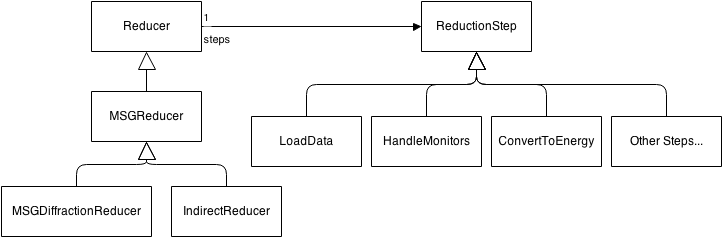
\includegraphics[width=1\textwidth]{img/uml/class_diagrams/Reducer_structure.png}
\caption{Diagram showing the class structure for the inelastic reducers and accompanying reduction steps.}
\label{fig:reducer-structure-diagram}
\end{figure}

Figure \ref{fig:reducer-structure-diagram} shows the class structure of indirect reducers and a subset of the reduction steps that are defined for inelastic energy reduction. In indirect data analysis we have two concrete reducer objects. One for energy conversion (IndirectReducer) and one for diffraction reduction (MSGDiffractionReduction). This section will just focus on the IndirectReducer. For discussion on diffraction reduction see section \ref{subsec:indirect-diffraction}.

The IndirectReducer object defines what steps should be executed as part of a reduction work-flow and is the point at which the parameters gather from the user interface are passed to the program. After setting up the each reduction step with the relevant parameters, the reducer then iterates over the list of steps and executes each one in turn on the sample run to be reduced. Reducer objects also have the option to define a preprocessing function which is only executed once regardless of the number of runs being processed. The MSGReducer, which is the superclass of both the IndirectReducer and the MSGDiffractionReducer, uses this to execute the loading step to get the sample run(s) to be reduced into memory before continuing with the rest of the reduction on a per run basis.

\begin{figure}[H]
\centering
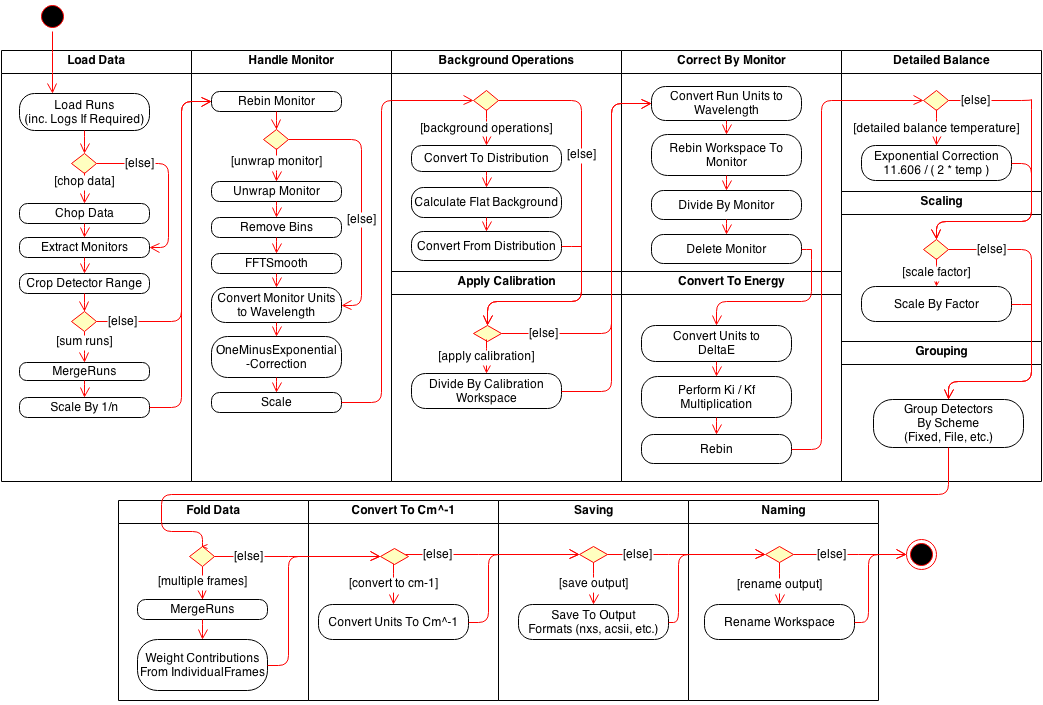
\includegraphics[width=1\textwidth]{img/uml/activity_diagrams/EnergyTransfer_activity.png}
\caption{Activity diagram showing the flow of execution for energy transfer reduction in release 3.2.}
\label{fig:c2e-energy-transfer-activity-diagram}
\end{figure}

The steps involved in energy transfer reduction are shown in activity diagram \ref{fig:c2e-energy-transfer-activity-diagram} along with the major operations performed within each step and the flow of the execution of the reduction. The responsibility of each of the steps are as follows:

\begin{itemize}
\item \textbf{Load Data} - The load data step loads each individual sample runs from file using the correct loader for the currently selected instrument. If the option is selected, it will also attempt to load the logs for the runs as well. If the current instrument has the parameter Workflow.ChopDataIfGreaterThan defined as in its instrument parameter file (IPF), the reduction step splits the data into multiple frames using the ChopData algorithm. The routine will then extract the monitor from the loaded workspace and crop the workspace to the desired detector range. If the sum option is checked the runs will be merged into a single workspace and averaged, otherwise subsequent steps are executed on each run individually.

\item \textbf{Handle Monitor} - Next the reducer prepares the monitors for correction later. This involves rebinning the monitor according to the step size defined the the IPF If. Next it will unwrap the monitor, if required, using the UnwrapMonitors algorithm to convert the workspace to have common bins within the maximum wavelength range given a reference flightpath between source, sample and first detector. It then tidies up the monitor by removing the bin at the joining wavelength and smooths it Using FFTSmooth. Finally it converts the units of the workspace to wavelength, performs an exponential correction for the thickness, attenuation and area of the monitor and scales it if a scaling factor is defined in the IPF.

\item \textbf{Background Operations} - This step simply calculates a flat background for the detectors data if parameters are defined for the background range and calculates the mean of the bins in this range before dividing by the width of the x range.

\item \textbf{Apply Calibration} - If a calibration file was supplied as a parameter for the reduction, the reducer will divide the workspace by the calibration run at this point. This just uses the standard Mantid Divide algorithm.

\item \textbf{Correct By Monitor} - The reducer then corrects the workspace by the preprocessed monitor by converting the units to wavelength then rebinning it to and dividing it by the monitor.

\item \textbf{Convert To Energy} - The conversion of the workspace to units of energy is then performed and multiplied by ki / kf , to transform the differential scattering cross section into a dynamic structure factor. The workspace is then rebinned according to the user defined rebin string.

\item \textbf{Detailed Balance} - The detailed balance step converts performs an exponential correction on the data if a temperature parameter was defined by the user.

\item \textbf{Scaling} - This step will scale the workspace by an arbitrary factor supplied by the user.

\item \textbf{Fold Data} - If the data was split into multiple frames during the loading step, the fold data step is performed. The individual frames are merged back into a single workspace and the workspace is scaled by averaging the contributions of each individual frame across the x range.

\item \textbf{Convert To $Cm^{-1}$} - If the option was selected, the workspace is convert to units of wavenumber.

\item \textbf{Saving} - If any save options were selected, the reduced workspace is saved in the desired format.
\item \textbf{Naming} - Finally, the reduced workspace is renamed according to the instrument-analyser-refection convention used in Mantid indirect inelastic.
\end{itemize}

Note that the instrument parameters used in energy transfer reduction are defined in files called \seqsplit{instrument\_name\_Parameters.xml} and \seqsplit{ instrument\_name\_analyser\_reflection\_Parameters.xml} where the instrument name, analyser, and reflection are replaced by the actual values used (e.g. IRIS\_graphite\_002\_Parameters.xml and are kept in the instrument directory within the Mantid installation directory.

\subsection{Calibration}
\label{subsec:c2e-calibration}
The calibration section of the convert to energy interface can be used to create calibration and resolution files using vanadium sample runs which can be used as part of data reduction and analysis. Calibration workspaces are generated by creating an executing a single reduction step object  (without creating a reducer object) called CreateCalibrationWorkspace. The procedure for generating a single calibration step is to load the runs, and if there is more then one of them merge them and scale the output workspace by a factor of $1/\,number\,of\,runs$. It then calculates a flat background based on a background range supplied by the user. The routine then integrates over the peak range (again, supplied by the user) and scales the resulting workspace. An activity diagram for the routine is shown in figure \ref{fig:c2e-calibration-activity-diagram}.

\begin{figure}[H]
\centering
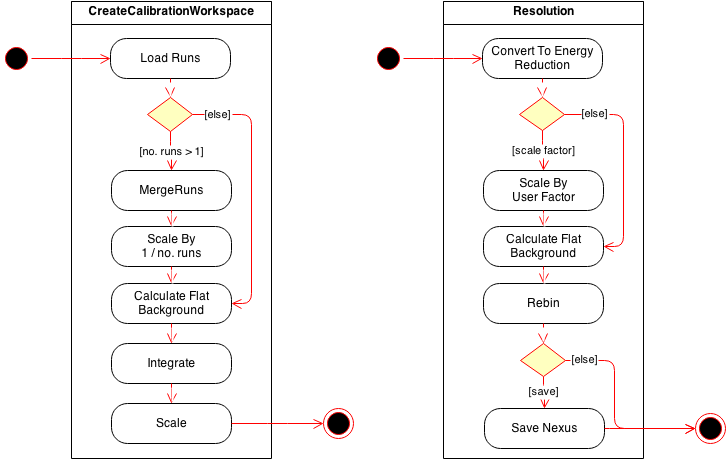
\includegraphics[width=0.6\textwidth]{img/uml/activity_diagrams/Calibration_activity.png}
\caption{Activity diagram showing the major steps of execution performed when creating a calibration and resolution workspace.}
\label{fig:c2e-calibration-activity-diagram}
\end{figure}

As mentioned, the calibration interfaces can also create resolution files for later use in data analysis. This routine, like many within the indirect section of many, is separate from the reducer-reduction step  framework and just a python function which is executed with parameters supplied from the interface. To create the resolution file, the routine first takes the vanadium run supplied on the calibration interface and converts it to energy using the energy transfer reducer described in section \ref{sec:energy-transfer}, but sets the detector mapping use all detectors and will sum multiple run if multiple runs are used. It then, like calibration, calculates a flat background from a range supplied by the user, rebins it according to the parameters specified for the instrument, and optionally saves the workspace to file.

\subsection{Diffraction}
Along side the energy transfer reduction Mantid also has an interface for the reduction of data from the diffraction experiments. The diffraction reduction implementation is based on the same reduced model that is used for energy conversion, but the number and complexity of the steps involved as part of the reduction are dramatically simpler than those used in energy conversion. 

\subsection{Diagnostics}
The diagnostics routine provides an integration on a run over a specified time-of-flight range. This routine loads the raw file and a calibration file (if requested) and integrates the resulting workspaces. If two ranges are requested, the second range is used to calculate a flat background and remove this from the data before integrating. Finally, the integrated workspace is then transposed to make it easier to visualise.

\subsection{Transmission}
The transmission routine is a simple program to calculate the measured transmission of a sample using the incident and transmission monitors. Using a run of both the sample and the can, monitors from each  raw file are extracted and converted to units of wavelength. The transmission monitor is then normalised by the incident monitor in each run over the common wavelength range. Finally, the sample is divided by the can to give the sample transmission as a function of wavelength.

\subsection{$S(Q,w)$}
In this interface, reduced files created as part of an energy transfer reduction can be converted to $S(Q,w)$. The Mantid framework has a collection of three algorithms that are used to convert a workspace from energy transfer to $S(Q,w)$ depending on the choice of rebinning to use. The mapping between $S(Q,w)$ algorithms and the rebin types are given in table \ref{table:sofqw-algorithms}. The code running an $S(Q,w)$ conversion is entirely contained within the Indirect interface where it dynamically builds a string of python code that is then executed. Optionally, the user many rebin the workspace in energy before hand. In this case, the routine simply calls the rebin algorithm with given parameters.

\begin{table}[H]
\begin{center}
\begin{tabular}{ c c}
Rebin Type & Algorithm Used \\ \hline
Centre & SofQW \\
Parallelepiped & SofQW2 \\
Parallelepiped / Fractional Area & SofQW3 \\
\end{tabular}
\caption{Table showing the relationship of rebin types to SofQW algorithms}
\label{table:sofqw-algorithms}
\end{center}
\end{table}

\subsection{$S(Q,w)$ Moments}
This is a new addition in Mantid 3.2 and provides a simple routine for calculating the first five statistical moments of an $S(Q,w)$. This is implemented as a standard Mantid algorithm (SofQWMoments) which is created and called from the interface though the algorithm manager and produces a group workspace with one workspace for each moment for every detector which has been transposed in order to make visualisation of the workspace easier.

\subsection{Support for the ILL}
The convert to energy reduction currently supports instrument at ISIS and the SNS. In release 3.2 a lot of work has been done in order to increase the level of support for ILL instruments. Prior releases of Mantid added a loader for ASCII data files from the ILL to the Indirect Load ASCII interface and stored in the file IndirectNeutron.py. In 3.2 loaders for various ILL instruments (including the very useful LoadILLIndirect) have been added. Additionally, a new reduction algorithm for IN16B, called IndirectILLReduction, has been to give support for energy transfer reduction within Mantid. Future releases aim to integrate this algorithm into the current reduction chain and therefore complete remove Indirect Load ASCII from the system.

\subsection{Energy Transfer GUI Overview}
Figure \ref{fig:c2e-class-diagram} shows the class structure of the indirect convert to energy. Note that for clarity only the more important methods and attributes are shown as part of the class diagram. The Convert to Energy window (for both direct and indirect instruments) inherits from Mantid's generic UserSubWindow class which provides the basic functionality required to render a sub window within the application and also provides some useful helper methods such as the ability to execute a string as a python script.

The ConvertToEnergy class itself contains the code which is shared between both direct and indirect versions of the interface. It is responsible for the loading the appropriate instrument definition files as the user selects an instrument, swapping between the indirect and direct interfaces depending on the geometry of the selected instrument, and handling the major user actions such as clicking the run energy transfer and help buttons.

\begin{figure}[H]
\centering
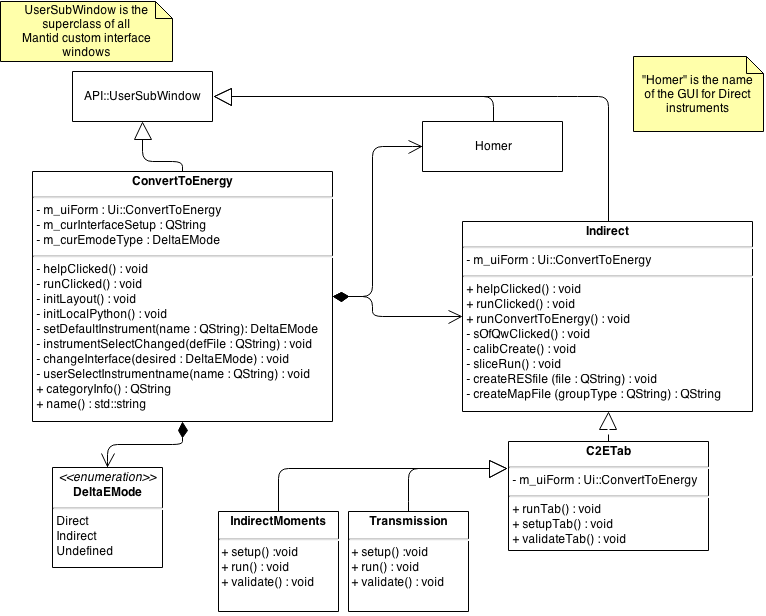
\includegraphics[width=0.8\textwidth]{img/uml/class_diagrams/C2E_structure.png}
\caption{Class diagram showing the structure of the Indirect Convert To Energy GUI in release 3.2.}
\label{fig:c2e-class-diagram}
\end{figure}

ConvertToEnergy is composed with two classes called Homer and Indirect that handle the functionality of direct and indirect geometry instruments respectively. In previous releases of Mantid the Indirect class contained all of the GUI code for every tab on the Indirect Convert To Energy interface. This is no longer the case in more recent versions of Mantid which have moved towards a more modular class structure.

As of release 3.2, the Indirect class contains the GUI code for the Energy Transfer, Calibration, Diagnostics, and S(Q,w) tabs. For each of these tabs there are corresponding methods (which are inconsistently named) to validate the user's input for that tab and run the appropriate routine. The specifics of each of these routines is outlined in the following sections. In order the execute the required routine, the GUI code for a particular tab builds a string which represents an executable python script complete with the options collected from the interface that can be executed using the runPythonCode() method inherited from UserSubWindow.

The actual design of the GUI is stored in a separate xml file that was created using Qt Designer and is used to produce a dynamically generated class for the interface at compile time which includes all the interface widgets for ConvertToEnergy. The ConvertToEnergy, Homer, and Indirect classes each have a reference to a copy of this interface object which they can query at runtime. The ConvertToEnergy class is responsible for adding and removing the appropriate tabs as the user switches between instrument geometries. The Indirect class uses this reference to query user input and update the interface appropriately in response to user actions.

In the past year there have been two additional tabs added to the Convert To Energy interface which do not follow the monolithic class structure current used by the majority of tabs in the indirect energy conversion interface. Instead of adding the code for the additional tabs IndirectMoments and Transmission directly into the Indirect class, a new class was created called C2ETab which is composed with the Indirect class (see diagram \ref{fig:c2e-class-diagram}). The specific implementations of the two new tabs are then handled by a specific class derived from the abstract C2ETab.

This approach is similar to the one already place in the Indirect Data Analysis interface (see \ref{subsubsec:IDA-GUI-Overview}) and provides a number of benefits over the initial design. Structuring the code in this way allows for greater modularity because each subclass of C2ETab is only concerned with the functionality relating to a single tab on the interface.

Furthermore, this design still allows code that is common between multiple tabs (such as code for plotting a histogram in a mini-plot) to be written once and shared across all classes through inheritance. Note that C2ETab also has a reference to the UI object so that it can interact with the widget objects defined on the interface, however this could easily be changed to use tab orientated interface objects (like the approach used by IndirectBayes, see \ref{subsubsec:Bayes-GUI-Overview} and further discussion in \ref{subsec:GUI-Improvements}) instead of having unrestricted access to the whole interface.

\subsection{Diffraction Reduction}
\label{subsec:indirect-diffraction}
Another key part of data reduction is the ability to reduce diffraction data. The process of preparing diffraction runs for analysis is much simpler than an energy conversion reduction. Indirect diffraction reduction uses the same reducer system as described in section \ref{sec:energy-transfer} but uses the MSGDiffractionReducer object (see figure \ref{fig:reducer-structure-diagram}) and a different selection of reduction steps. 

The instrument parameters used in reduction are defined in files called \seqsplit{ \textit{instrument\_name}\_diffraction\_diff\_spec\_Parameters.xml} and \seqsplit{ \textit{instrument\_name}\_diffraction\_diff\_only\_Parameters.xml} (if the instrument supports diff only mode).

\begin{itemize}
\item \textbf{Load Data} - The first step in diffraction reduction is to load all of the data files to be reduced. This reduction step is exactly the same as the one described in section \ref{sec:energy-transfer}.

\item \textbf{Handle Monitor} - Next the reducer prepares the monitors for correction. Again the procedure for this step is exactly the same as the one described in section \ref{sec:energy-transfer}.

\item \textbf{Correct By Monitor} - Again this is the same as described in section \ref{sec:energy-transfer}, but instead when running the convert units algorithm to convert the workspace to wavelength the reduction step uses the Elastic energy mode option instead of Indirect energy mode option.

\item \textbf{Fold Data} - If the data was split into multiple frames during the loading step, the fold data step is performed. This is identical to section \ref{sec:energy-transfer}.

\item \textbf{Convert Units To $d$-spacing} - This is not a reduction step, but just a call to the Mantid ConvertUnits algorithm to covert the workspace to units of $d$-spacing with the energy mode used being elastic.

\item \textbf{Rebin} - If the a rebin string was supplied to the reducer, the workspace is rebinned according to the supplied parameters. Again this is not a reduction step but just a plain call to the Rebin . If not rebin string was supplied, the workspace is rebinned to the first spectrum using the reduction step of the same name. This step just calls the RebinToWorkspace algorithm with all arguments set to the workspace.

\item \textbf{Groping} - Next the grouping reduction step is performed, which is the same as in section \ref{sec:energy-transfer} but with the grouping type hard coded to simply show all spectra.

\item \textbf{SaveItem} - Finally, the reduced workspace is past through the SaveItem reduction step where the output options past to the reducer are processed. Once again, this step is identical to the one described in section \ref{sec:energy-transfer}.

\end{itemize}

\subsection{OSIRIS Diffraction Reduction}
The OSIRIS instrument uses a separate reduction algorithm called OSIRISDiffractionReduction for use in diff only mode and does not use the reducer chain. This algorithm takes a list of samples and a list of vanadium runs and an old style calibration (these are not the ones generated by the routine in section \ref{subsec:c2e-calibration}, but the type supplied to the AlignDetectors and DiffractionFocussing algorithms). Each of the sample/vanadium run pairs can cover a different $d$-range which the algorithm then merges using the MergeRuns algorithm. This algorithm proceeds as follows:

\begin{itemize}
\item The algorithm begins by loading all of the samples and vanadium runs into workspaces. This just uses the Load algorithm.

\item The algorithm then maps each of the supplied samples to there corresponding $d$-range and averages any workspaces that are in the same $d$-range. The same procedure is repeated for the vanadium runs.

\item At this point the algorithm has a processed list of all workspaces and their background for each $d$-range and can begin the reduction. The algorithm now Normalises by the beam current, aligns detectors and performs diffraction focussing using the calibration file provided, and then crops the workspace to match it's $d$-range. These operations are performed for each sample and vanadium run.

\item The background for the runs is then processed by rebinning each sample/vanadium pair to match and dividing the sample by the vanadium. Any NaN or Infinity values after this operation are replaced with zeros.

\item Finally all of the samples are merged into a single workspace using the MergeRuns algorithm and the workspace is scaled at the points of intersection where there are overlapping ranges.
\end{itemize}

\subsection{Indirect Diffraction GUI Overview}
The corresponding interface for diffraction reduction is called Indirect Diffraction. Unlike the other interfaces in the Indirect collection, the structure of this interface is just a single class with a single UI file defining the layout. Each instrument has either the option of running in Diff Spec or Diff Only mode (TOSCA and VESUVIO only have diff spec mode) and as described in the previous section OSIRIS has a different reduction routine in the case of diff only mode. This is reflected in the interface when the user selects the appropriate option. The GUI changes the way the interface looks by checking the instrument parameter files for the currently selected instrument and reflection.

\section{Data Analysis with Mantid}
After data has been reduced using the convert to energy or diffraction reduction routines described in the previous section the reduced data needs to be analysed. In the indirect section of Mantid, there are two major collections of data analysis scripts that are currently in place. The first  and most important are those included in the Indirect Data Analysis interface which provide a variety of different fit functions and transforms the can be performed on reduced data. The second collection of routines are accessible via the Indirect Bayes interface. This provides a collection of routines that can be used to infer fitting parameters using Bayesian model selection techniques which are complementary to the routines in Indirect Data Analysis.

The majority of the code for data analysis scripts can be found in the file IndirectDataAnalysis.py with the Inelastic script folder of the Mantid installation, with the exception of Calculate Corrections which is in a file called IndirectAbsCor.py. For the Bayesian fitting programs, the code is stored in the file IndirectBayes.py, with the exception of JumpFit which is stored in IndirectJumpFit.py both of which are in the Inelastic scripts folder.

\subsection{ElWin}
The ElWin (elastic window) program is used to perform elastic window scans by integrating over the energy range of a reduced file and is based on the routine of the same name that was originally provided as part of the MODES package. As with most all routines in the Indirect Data Analysis interface, the ElWin is implemented as a collection of free standing functions in IndirectDataAnalysis.py. Internally, this routine uses Mantid's ElasticWindow algorithm. This algorithm does most of the heavy lifting, while the script provided in IndirectInelastic.py pre and post processes the data. The elastic window algorithm converts the spectrum axis of the input workspace to units of $Q$ and $Q^2$. Both of these workspaces are then transposed so they are easier to visualise. Optionally, this routine can also remove a background using a second range.

The ElWin routine will attempt to output processed workspaces with units in Kelvin on the x-axis of the  providing that data about the temperature of the run is available as in the sample logs of the workspace (which are optionally loaded as part of energy transfer reduction). If this information is not available, the routine will use the run number of each sample for the units on the x-axis. If the workspaces have units of temperature, the routine can also optionally output the \**\_elf workspace normalised by the lowest temperature.

The $Q^2$ output for ElWin is used as the input to the MSDFit routine described in the following section.

\subsection{MSDFit}
The MSD fit routine is used to calculate the mean squared displacement from the $Q^2$ workspace output from ElWin. In essence this routine performs a linear fit to every spectrum in the workspace using the algorithm PlotPeakByLogValue. However the routine also performs some additional operations to transform the fitting parameters form a table workspace to a matrix workspace.

This routine produces a group workspace contain the linear fits to each spectrum and a workspace for each of the parameters of the fit to each spectrum transposed into a matrix workspace.

\subsection{Fury}
The Fury program is used to perform a fast Fourier transform on a reduced workspace in order to calculate the intermediate scattering function $I(Q,t)$. The routine can handle converting multiple workspaces at once, but is currently only set-up to handle the interface to convert one reduced sample at a time.

The routine first converts the resolution workspace before converting each of the samples and dividing by the converted resolution. In order to convert to the intermediate scattering function all of the workspaces must have the same x range and the same regular binning in order for the conversion to work. Therefore the rebin parameters provided by the user must satisfy these conditions. The workspace is then integrated to a separate workspace. The original workspace is then converted to point data in preparation for running the fast Fourier transform algorithm.

The algorithm used is called ExtractFTTSpectrum which runs Mantid's FFT algorithm to on each spectrum in the workspace which outputs the modulus positive frequencies of the transform in the corresponding spectrum. The transformed sample workspaces are then divided by the transformed resolution workspace. The upper half of the transform is then crop off of the workspace to get rid of excess noise from the transform and then optionally saved to a nexus file.

\subsection{FuryFit}
FuryFit provides a fit routine for the output of Fury offering a variety of decaying exponential functions. Similarly to MSDFit, the routine uses the Fit and PlotPeakByLogValue algorithms to sequentially fit each spectrum with the parameters.

The FuryFit code actually consists of two routines which are very similar and which could be merged in future release of Mantid called FuryFitSeq and FuryFitMult which perform a sequential fit and a multi domain fit respectively. Both routines works by executing a function string which is dynamically created in the GUI code for FuryFit, but FuryFitMult first wraps the input function with a MultiDomain composite function. FuryFitMult is only executed when the user has chosen to constrain the $\beta$ parameter for a stretched exponential fit across all $Q$.

Both of these routines convert the table of fitting parameters created from Fit (or PlotPeakByLogValue) into a matrix workspace using the same code as used by MSDFit.

\subsection{ConvFit}
The ConvFit routine is used to perform a convolution fit to the workspaces. Again, this routine follows a similar procedure to both the MSDFit and FuryFit routines. A fit function with the options the user has selected are gathered from the user interface and a string representing the function to be fitted is passed to the PlotPeakByLogValue algorithm to perform a sequential fit.

The functions fitted are a $\delta$-function, one or two Lorentzians or a combination of both which are then convolved with the user supplied resolution workspace. The type of background can also be selected from a choice of Fixed Flat (flat background without the intercept tied to the user supplied value), Fit Flat (flat background with the intercept unconstrained), and Fit Linear (unconstrained linear background). Optionally a temperature correction can be applied to the Lorentzians.

As with the other FuryFit, ConvFit will convert the input workspace to elastic $Q$ first before performing the fit, and converts the output table of fit parameters to a matrix workspace. If a $\delta$function was used the elastic incoherent structure factor (EISF) is calculated from the resulting table of parameters.

\subsection{Calculate Corrections}
Calculate Corrections is used to create a group workspace of absorption corrections from known parameters of the sample and can used in an experiment which can be applied to a reduced workspace using the Apply Corrections routine (see section \ref{subsubsec:apply-corrections}). This routine supports both flat plate and cylindrical geometries.

The code for calculating corrections for a cylindrical geometry is has been ported into Mantid using the F2Py package directly from it's previous incarnation as the Acorn routine in the MODES package. This allows a python script run the Fortran code without it being converted to python code. Unfortunately the downside to this is that F2Py cannot be packaged into the installer for any platform outside of Windows. The code for flat plate corrections was ported in Mantid as part of release 3.2.

In depth discussion on the exact methods of calculating the absorption factors for flat plate and cylindrical geometries can be found in Carlile \cite{ccarlile1974} and the ATLAS manual \cite{aksoper1989} respectively.

The python code underlying the interface of calculate corrections and responsible for liaising between the Fortran and C++ GUI code is (unlike the other routines described in this section) stored in a separate file called IndirectAbsCor.py. This is to keep F2Py import call separate from the rest of the data analysis code, so the other interfaces can be used on platforms other than Windows.

Regardless of the geometry used, the Python/Fortran code calculates four arrays for each spectrum in the sample workspace each of which are collected into four resulting output workspaces with the suffixes \textit{ass}, \textit{assc}, \textit{acsc}, and \textit{acc} which loosely corresponds to the formalism described in Paalman and Pings \cite{hhpaalman1962}. These stand for:

\begin{itemize}
\item \textbf{Ass} - Attenuation factor for scattering in the sample and attenuation in the sample.
\item \textbf{Assc} - Attenuation factor for scattering in the sample and attenuation in the sample plus container.
\item \textbf{Acsc} - Attenuation factor for scattering in the container and attenuation in the sample plus container.
\item \textbf{Acc} - Attenuation factor for scattering in the container and attenuation in the container.
\end{itemize}

If a workspace representing the container is not supplied by the user, then all workspaces except the \**\_ass workspace will just contain zeros.

\subsection{Apply Corrections}
\label{subsubsec:apply-corrections}

Apply Corrections provides a complementary routine to the calculate corrections routine described in the preceding section. Apply corrections has two modes of applying corrections to a sample. The first and simplest method is to just take a run of the container for the sample and subtract it from the sample itself. The second uses the corrections calculated from the calculate corrections routine and applies them to the sample \& can workspaces. A detailed activity diagram of the two modes of execution are shown in diagram

In the former mode of operation if the energy ranges of the sample and container do not match the user gets offered the choice of rebinning the can to match the sample in which case the routine uses the RebinToWorkspace algorithm. After the sample has been corrected, it will use the ConvertSpectrumAxis algorithm to convert the resulting corrected sample to units elastic Q.

In the latter mode of operation, the routine first converts both the sample and container to units of wavelength. Then for spectrum in the sample and can (if supplied), perform a quadratic fit (using the standard Mantid Fit algorithm) to the corresponding spectrum in each of the members of the group workspace of absorption corrections. The coefficients from this fit are then supplied as parameters to the PolynomialCorrection algorithm. The resulting workspaces are then stitch back together using the ConjoinWorkspaces algorithm and the corrected can is then subtracted from the sample workspace as in simpler mode of apply correction. The output from function is output both in units of energy transfer and elastic Q.

\subsection{GUI Overview}
\label{subsubsec:IDA-GUI-Overview}
The Indirect Data Analysis user interface follows a similar design structure to the Convert To Energy interface but is more modular. The interface is composed of a single which handles the common aspects between all tabs on the interface, which is simply called Indirect Data Analysis, and a collection of classes for each tab on the interface which inherit from a common base class similar to the C2ETab class in the convert to energy GUI and handle the specific implementation details of the corresponding tab.

As with the convert to energy interface, the layout of the entire GUI is defined in a single XML file which each of the classes in the GUI have a reference too. As of release 3.2 the Indirect Data Analysis interface consists of seven tabs; namely: ElWin, MSDFit, Fury, FuryFit, ConvFit, Calculate Corrections, and Apply Corrections. Each of these have a single class which inherits from a base class called IDATab where the common logic between individual classes is stored. 

\subsection{Indirect Bayes}

The Indirect Bayes interface provides a collection of routines for performing model and parameter selection using Bayesian methods. These routines are, like those in proceeding sections, based on those from MODES. The ResNorm, Quasi, and Stretch routines described in the following sections are all imported into Mantid using the F2Py package directly from the original Fortran code. 

In future releases of Mantid it is hoped that these routines will be converted into proper C++ or Python algorithms as with the rest of Mantid. The routines defined in here are included in Mantid in the file IndirectBayes.py and the accompanying Fortran modules which are in the same folder. The majority of the code in this file does not currently use standard Mantid algorithms, largely because the the Fortran code obviously doesn't work with workspaces and so we are reduced to working with numpy arrays. Worse than this, in the Quasi fitting routine the fit parameters get written to file, which is then immediately read back into the program.

\subsection{ResNorm}
ResNorm is used to create a group normalisation workspace which can be input to Quasi (described in the next section). It normalises the input data using the instrument resolution by fitting. A group normalisation may also be done by grouping Q values where the resolution is stretched using a stretch factor. The routine produces two group workspaces with the suffixes \**\_ResNorm and \**\_ResNorm\_Fit respectively. The ResNorm group workspace contains two workspaces with the suffixes intensity and stretch. The intensity workspace contains the intensity normalisation factor and stretch contains a stretch factor for the width of the supplied resolution file. The ResNorm\_Fit group workspace contains the fits to each spectrum in the workspace.

\subsection{Quasi}
The Quasi routine provides a model selection algorithm using Bayesian methods to choose the number of lorentzian components present in the input data \cite{dssivia1992} and was originally known as Quasi Lines in the old MODES package. This routine takes a sample to fit to and a resolution file created in the convert to energy interface and optionally a resolution normalisation file created in ResNorm (see the previous section). This program can run either by fitting a $\delta$-function plus a sum of Lorentzians or a single stretched exponential. There are three Fortran modules which are used depending on the input. The QLres module fits a sum of Lorentzians. If the resolution file contains more than one spectrum, then the QLdata module is used and any ResNorm file supplied is ignored. Finally if the choice of fitting a stretched exponential is used the QLse module is used. Each of these modules share very similar code which is duplicated and modified slightly to suit the specifics of the implementation.

Inside the fitting routine it first refines the parameters for the $\delta$-function, linear background, energy range offset and thereby estimates probability of the absence of quasielastic components in data. It then refines the parameters for one, two and three Lorentzian components successively \cite{dssivia1992}.

Internally the program loads both the ResNorm and width files into 1D arrays. It then extracts from the sample and resolution workspaces a the x, y, and e arrays for each spectrum in the workspace and passes this data to the Fortran routine with any accompanying fit parameters used. The corresponding fits to the data are returned in the form of x, y, and e arrays for the spectrum and its log probability for each Lorentzian (from 0 to 3). Additionally, the program also reads the program parameters from the generated file (saved in the user's default save directory) and creates a workspace of fit parameters similar to the one output by ConvFit. Likewise, it will also calculate the EISF from the fit parameters.

\subsection{Stretch}
Stretch is a variation on stretched exponential option provided by the Quasi program described in the previous section and was originally called Quest in the old MODES package. The Fortran module used is called Que. The operation of the two programs are essentially the same, except that a grid of $\beta$ and $\sigma$ parameters are fitted to each spectrum instead.

This fit routine produces one group workspace containing the fit to the data for each spectrum and two additional workspaces containing the parameters $\beta$ and $\sigma$ parameters of the fit.

\subsection{JumpFit}
JumpFit provides very simple routine for fitting the width parameters fitted to a workspace from either Quasi or ConvFit. It offers a collection of diffusion fit functions (defined as python fit functions). The desired component width and function type is selected by the user, a fit function string is built and passed to the Mantid's Fit function. The fit functions used in JumpFit are currently hard coded to use the default values shown in table \ref{table:jumpfit-functions}.

\begin{table}[H]
\begin{center}
\begin{tabular}{ l l l}
Function & Function Definition & Default Parameter Values \\ \hline
Chudley-Elliot &  $Gamma(Q) = (1 - sin(Ql)/Ql)/\tau$ & $\tau = 1.0/QMax, L=1.5$\\ \hline
Hall-Ross & $ Gamma(Q) = (1-exp(-l*Q^2))/\tau$ & $\tau = 1.0/QMax, L=1.5$ \\ \hline
Fick & \parbox{6cm}{$Gamma(Q) = D*Q^2$ \\ where $D=<l^2>*Q^2/6*\tau$} & $D = \Delta y / \Delta x^2$\\ \hline
Teixeira Water & \parbox{6cm}{$Gamma(Q) = D*Q^2/(1 + D*Q^2*\tau)$ \\ where $D=<l^2>*Q^2/6*\tau$} & $\tau = 1.0/QMax, L=1.5$ \\ \hline
\end{tabular}
\caption{JumpFit function names, definitions, and default parameter values.}
\label{table:jumpfit-functions}
\end{center}
\end{table}

\subsection{GUI Overview}
\label{subsubsec:Bayes-GUI-Overview}
The GUI structure for the Bayes interface again follows a similar structure to the convert to energy and indirect data analysis interfaces, but takes the abstraction a step further. Like the interfaces discussed before this interface has a single parent class called IndirectBayes which defines the window and a collection of concrete classes paired with each of the tabs which inherit from an abstract base class called IndirectBayesTab which implements the common functionality each tab. 

The key difference between the two is that instead of the interface being defined in a single UI file, the main window and each of the tabs are defined in separate UI files. This is a subtle difference, but one which provides an enormous benefit to the development process. Splitting the UI into multiple files makes the interface more maintainable as tab can be worked on individually without affecting the others.

\section{Simulation}
Another important part of experimental analysis involved the comparison of actual results against theoretical predictions. This is an area of development that is only just beginning and there is only a very small amount of support implemented so far.

\subsection{Indirect Simulation}
Indirect Simulation is a new interface for release 3.2 that splits the basic nMolDyn loader that is currently in Mantid off from it's original location in the Indirect Load ASCII interface. This interface is planned to be a place to expose simulation routines to the GUI with plans to add support for the Sassena routines already in Mantid planned in future releases.

\subsection{nMolDyn}
The nMolDyn interface that currently exists is a very simple routine load data from a nMolDyn simulation files into a Mantid workspace. In future releases of Mantid it is proposed to attempt to properly integrate support for the nMolDyn python libraries into Mantid, providing a much richer array of tools for the user. The code for this can be found the IndirectMolDyn.py file in the Inelastic scripts folder.

\subsection{Density Of States}
The Density of States algorithm is does not currently have GUI support, but was a new addition to the 3.1 release of Mantid. It provides loading algorithm for .castep and .phonon files generated by CASTEP simulation program and create workspaces with both total and partial density of states data. Further support for CASTEP is planned in future releases. The code for this file can be found in DensityOfStates.py file under python algorithm plugins section in the Mantid install.

\section{Planning For the Future}
This section outlines outstanding work in pertaining to support of Indirect geometry instruments within Mantid. This section is not meant as a "set in stone" plan for further development but is meant as guide for future development work in the area and a loose record of user and project requirements which are subject to change.

\subsection{Conversion of Existing Routines to Algorithms and Work-Flow Algorithms}
Now that a large proportion of the code base required for data reduction and analysis of Indirect geometry spectroscopy has been incorporated into Mantid, it is time to move forward with consolidating the existing code base we already have. As already mentioned in the earlier sections of this document most of the code base is either using the old style reducer-reduction step framework or is in the form of simple python scripts which are both not sufficiently documented and (largely) untested.

Ideally, the Indirect framework should take advantage of the core concept of the Mantid framework: algorithms. An algorithm in Mantid is defined as being a set of code that performs some operation on a workspace of data. Algorithms are well documented (both for the user and the development team) and are the preferred common interface for performing actions in Mantid.

There are two types of algorithms in Mantid. Normal algorithms are simply ones which perform some operation on a workspace, such as ConvertUnits or Fit or Load. The second type is called a work flow algorithm. This is an algorithm that performs no direct manipulation of a workspace itself, but is a collection of algorithms that perform some larger task. The benefits of the latter are that: 

\begin{itemize}
\item Large operations get broken do into smaller, more easily understood operations which already have algorithm defined which are used by multiple research groups and facilities and have become tried and tested.

\item Algorithms and Work flow algorithms still support inheritance like the reducer objects

\item They are easily unit testable, meaning that automated checking of the integrity of each part of the reduction is handled automatically by the build servers, which helps prevent errors.

\item They are by default exposed through the Mantid simple python API like any other algorithm which means they can easily be chained together with other algorithms and can be run even if the interface is broken.

\item As of release 3.2 the ability to track the history of a work flow algorithm and it's child algorithms has been added, allowing scientists to see exactly what operations have been performed on a workspace since it entered Mantid.
\end{itemize}

Energy transfer reduction and diffraction reduction are both prime candidates for work flow algorithms. Neither of these routines actually perform any real direct manipulation of the workspaces they reduce themselves, but delegate all of the operations to existing Mantid algorithms within the reduction steps. Converting this would be a delicate and large job, but not necessarily difficult. The basic outline of both reductions is already documented in diagrams \ref{fig:c2e-energy-transfer-activity-diagram} and \ref{•} respectively. This, along with the actual code (which is reasonably we documented and formatted) should be enough for an easy transition to a work flow algorithm for each type of reduction.

Some of the large reduction steps would also benefit from being converted to work flow algorithms in there own right, particularly the reduction steps which are larger and shared between both reducer classes. Prime examples would be the LoadData and HandleMonitor steps which both complex enough that they could be converted to work flow algorithms.

To convert the existing reduction routines into work flow algorithms, I would suggest first writing detailed unit tests to cover all of the reduction steps. The energy conversion itself is already covered by automated system testing to periodically check the integrity of the results. The next step would be to concrete reducer classes to be algorithms one at a time and hooking them up with the relevant GUI. The final step would be to convert the reduction steps to either be algorithms or work flow algorithms in there own right or to simply incorporate the code into the reduction work flows themselves. Work flow algorithms essentially just a class and therefore support inheritance which means common code between both reducers should end up being stored in a common base class.

Outside of the main reducers, the main other scripts used throughout the Indirect framework should be converted to be proper Mantid algorithms for the reasons listed above. However, many of these routines are considerably simpler than the reducer work flows and many of them may be best just being converted to plain algorithms. Many routines, such as the the data analysis fitting routines MSDFit, FuryFit and ConvFit share very functionality with only a few slight difference between implementations. In the case of the routines listed, essentially passes a function string to PlotPeakByLogValue or Fit and converts the output table workspace to a matrix workspace of parameters. These could probably be reimplemented as a single algorithm with handles the fitting for all three routines. Consolidating the code base in this way could also be done with the Bayesian fitting routines Quasi and Stretch but should only be done after converting the Fortran modules (see section \ref{subsec:convert-fortran}).

\subsection{Better Automated Test Coverage}


\subsection{Improved GUI structure and design}
\label{subsec:GUI-Improvements}

%\subsection{GUI support for VESUVIO}
\subsection{nMOLDYN integration into Mantid}
\subsection{Conversion of Remaining Fortran Routines}
\label{subsec:convert-fortran}
As mentioned in several sections through out the documentation of existing development, are several routines that still rely on Fortran routines that have been directly assimilated into Mantid using the F2Py package. This has allowed quick integration of routines needed for analysis, it is not a cross platform solution, is not well documented, and is difficult to decipher.

A long term goal would be to convert these existing, tried and tested routines into well documented, thoroughly unit tested C++ code which utilises the existing some of the fitting routines that we already have inside Mantid. As mentioned in the previous section, some of the functionality is repeated inside the code for Quasi and Stretch and it may be the case that common code could be shared during the conversion.

The biggest difficulty with this is that it will require a sizeable chunk of a developers time and a good understanding of Fortran to convert the routines and write thorough tests for the converted code to ensure the fitting is good enough to match the existing Fortran while still matching the process described in the references \cite{dssivia1992}.

There are currently four routines that are still in Fortran code: the three Bayes programs and the cylindrical absorption corrections program used in the calculate routine. There are additional Fortran based routines in the for multiple scattering (see section \ref{subsec:multiple-scattering}) which will also need to be ported to Mantid in future releases.

\subsection{Improved Support for Other Facilities}
\subsection{Multiple Scattering Support}
\label{subsec:multiple-scattering}
The multiple scattering routines from the MODES package are the last major parts that have not been ported from the MODES application in one form or another. There are two different multiple scattering routines called MuscatData and MuscatFunc.

\bibliographystyle{plain}
\bibliography{refs}
\end{document}
